\documentclass[11pt,a4paper]{article}
\usepackage{examgrid}
\setdoc{Allocation Algorithm and Backend Specification}{EG-DOC-03}
\newcommand{\src}{../../src/main/java/com/examgrid}

\begin{document}
\nmamitcover{Allocation Algorithm and\\Backend Specification}{Document 03 of 05 \,\textbullet\, Seating and Invigilation Rules, Exception Handling, Security}{\small Department of Computer Science and Engineering\\[6pt]November 2026}

\pagenumbering{roman}
\doccontrol{EG-DOC-03}{Approved baseline}
\newpage
\tableofcontents
\newpage
\pagenumbering{arabic}

\section{Introduction}
This document specifies the core of ExamGrid: the rule-based \textbf{seating allocation engine} and the \textbf{invigilation allocation engine}, together with the backend mechanisms that protect them -- transactions, validation, centralized exception handling and Spring Security. Every listing in this document is included directly from the project source code, so the document and the implementation cannot drift apart.

\section{Problem Formulation}
\subsection{Inputs}
\begin{itemize}
  \item A slot $T = (d, t_s)$: all exams $E = \{e_1, \ldots, e_k\}$ with date $d$ and start time $t_s$.
  \item For each exam $e_i$, the set of students $S_i$ of its branch and semester, $n_i = |S_i|$, $N = \sum n_i$.
  \item Halls $H = \{h_1, \ldots, h_m\}$; hall $h_j$ has $r_j$ rows and $c_j$ columns, capacity $C_j = r_j c_j$.
  \item Faculty $F$; faculty $f$ has a duty limit $L_f$ and a set of already assigned duties $D_f$.
\end{itemize}

\subsection{Hard Constraints (must never be violated)}
\begin{enumerate}[label=\textbf{H\arabic*}]
  \item Every student of every exam in the slot gets exactly one seat.
  \item At most one student per physical seat; seats used in hall $h_j$ $\le C_j$.
  \item If $N > \sum_j C_j$ the allocation is refused.
  \item A faculty member never holds two duties whose time intervals overlap on the same date.
  \item A faculty member never exceeds $L_f$ duties.
  \item Each used hall with $s$ students gets $\lceil s/30\rceil$ invigilators (minimum 1).
\end{enumerate}

\subsection{Soft Constraints (satisfied whenever space allows)}
\begin{enumerate}[label=\textbf{S\arabic*}]
  \item Two horizontally or vertically adjacent students do not write the same subject.
  \item Adjacent students preferably belong to different branches.
  \item Invigilation workload is balanced: $\max_f |D_f| - \min_f |D_f|$ is as small as possible.
\end{enumerate}

\subsection{Choice of Approach}
Exact methods such as backtracking or integer linear programming can guarantee optimality but their running time grows exponentially and they are hard to explain in a lab viva. A greedy algorithm that picks, seat by seat, the \emph{largest waiting group that does not clash with the already placed neighbours} is linear in the number of seats, always satisfies the hard constraints, and in practice satisfies S1 completely whenever the slot contains two or more subjects or there are spare seats. The same greedy idea -- \emph{least-loaded free faculty first} -- solves the invigilation problem.

\section{Seating Allocation Engine}
\subsection{Seat Neighbourhood}
Seats are filled row by row from the blackboard (row 1, column 1) to the back of the hall. When seat $(r, c)$ is filled, its \emph{left} neighbour $(r, c-1)$ and \emph{front} neighbour $(r-1, c)$ are already decided, while the right and back neighbours will be checked when they are filled. Therefore checking only left and front is sufficient to guarantee that no two adjacent seats hold the same subject.

\subsection{Algorithm}
\begin{algorithm}[H]
\caption{Greedy seating allocation for one slot}
\begin{algorithmic}[1]
\Require slot date $d$, start time $t_s$
\State $E \gets$ exams with date $d$ and start $t_s$; \textbf{if} $E = \emptyset$ \textbf{throw} AllocationException
\For{each exam $e \in E$} \State $Q_e \gets$ queue of students of $e$'s branch and semester ordered by USN \EndFor
\State $N \gets \sum |Q_e|$; $H \gets$ halls sorted by capacity descending; $C \gets \sum$ capacity
\If{$N > C$} \State \textbf{throw} InsufficientCapacityException$(N, C)$ \EndIf
\State delete existing seats and duties of the slot
\State $remStudents \gets N$; $remSeats \gets C$; $clashes \gets 0$
\For{each hall $h \in H$ \textbf{while} $remStudents > 0$}
  \For{each seat $(r, c)$ in row-major order \textbf{while} $remStudents > 0$}
    \State $L \gets grid[r][c-1]$; $F \gets grid[r-1][c]$
    \State $e \gets$ \Call{PickExam}{$L, F$, avoidBranch = true}
    \If{$e = $ null} \State $e \gets$ \Call{PickExam}{$L, F$, avoidBranch = false} \EndIf
    \If{$e = $ null}
       \If{$remSeats > remStudents$} \State leave seat empty; $remSeats \gets remSeats - 1$; \textbf{continue} \EndIf
       \State $e \gets$ exam with largest $|Q_e|$; $clashes \gets clashes + 1$
    \EndIf
    \State $s \gets Q_e.\mathrm{poll}()$; $grid[r][c] \gets e$; record seat $(e, s, h, r, c)$
    \State $remStudents \gets remStudents - 1$; $remSeats \gets remSeats - 1$
  \EndFor
\EndFor
\State save all seats; \Return SeatingResult$(d, t_s, |E|, N, hallsUsed, clashes)$
\Statex
\Function{PickExam}{$L, F$, avoidBranch}
  \State \Return the exam $e$ with the most waiting students such that $|Q_e| > 0$, $e \ne L$, $e \ne F$ and, if avoidBranch, branch$(e) \ne$ branch$(L)$ and branch$(e) \ne$ branch$(F)$
\EndFunction
\end{algorithmic}
\end{algorithm}

\begin{figure}[H]\centering
\resizebox{!}{0.62\textheight}{\begin{tikzpicture}[
  font=\footnotesize, node distance=0.45cm,
  term/.style={rounded rectangle,draw=egnavy,fill=egnavy,text=white,minimum height=0.7cm,minimum width=3cm},
  proc/.style={rectangle,draw=egnavy,fill=eglight,rounded corners=2pt,minimum height=0.7cm,text width=5.2cm,align=center},
  dec/.style={diamond,draw=eggold,fill=eggold!20,aspect=2.6,inner sep=1pt,text width=2.8cm,align=center},
  err/.style={rectangle,draw=red!60!black,fill=red!8,rounded corners=2pt,text width=3.2cm,align=center,minimum height=0.7cm},
  arr/.style={-{Stealth[length=2mm]},thick}]
\node[term] (s) {Start (date, startTime)};
\node[proc,below=of s] (p1) {Load exams of the slot; build one waiting queue of students per exam (branch + semester)};
\node[dec,below=of p1] (d1) {students $>$ total hall capacity?};
\node[err,right=0.8cm of d1] (e1) {throw InsufficientCapacity\-Exception};
\node[proc,below=of d1] (p2) {Delete old seats and duties of the slot; sort halls by capacity (largest first)};
\node[proc,below=of p2] (p3) {For each hall, for each seat (row by row): read left and front neighbour};
\node[proc,below=of p3] (p4) {Pick exam with most waiting students whose subject \emph{and} branch differ from both neighbours};
\node[dec,below=of p4] (d2) {found?};
\node[proc,right=0.8cm of d2,text width=3.4cm] (p5) {Relax: only subject must differ};
\node[dec,below=of d2] (d3) {found?};
\node[dec,left=0.8cm of d3,text width=2.2cm] (d4) {spare seats left?};
\node[proc,above=0.35cm of d4,text width=2.0cm] (skip) {leave seat empty};
\node[proc,below=of d3] (p6) {Place next student of chosen exam; record seat (row, column, label)};
\node[dec,below=of p6] (d5) {students left?};
\node[proc,below=of d5] (p7) {saveAll seats; return SeatingResult};
\node[term,below=of p7] (e) {End};

\draw[arr] (s)--(p1); \draw[arr] (p1)--(d1);
\draw[arr] (d1)--node[above]{yes}(e1);
\draw[arr] (d1)--node[right]{no}(p2);
\draw[arr] (p2)--(p3); \draw[arr] (p3)--(p4); \draw[arr] (p4)--(d2);
\draw[arr] (d2)--node[right]{yes}(d3);
\draw[arr] (d2)--node[above]{no}(p5);
\draw[arr] (p5) |- (d3);
\draw[arr] (d3)--node[right]{yes}(p6);
\draw[arr] (d3)--node[above]{no}(d4);
\draw[arr] (d4)--node[right]{yes}(skip);
\draw[arr] (d4) |- node[pos=0.25,left,align=right]{no: place\\anyway,\\clash++} (p6.west);
\draw[arr] (skip.north) |- (p3.west);
\draw[arr] (p6)--(d5);
\draw[arr] (d5)--node[right]{no}(p7);
\draw[arr] (d5.east) -- node[above]{yes} ++(4.8,0) |- (p3.east);
\draw[arr] (p7)--(e);
\end{tikzpicture}
}
\caption{Flowchart of the seating allocation engine}
\end{figure}

\subsection{Why Largest Group First}
Choosing the exam with the most waiting students keeps the queues balanced. If small groups were used first, the last rows of the last hall would contain only the biggest subject and same-subject neighbours would become unavoidable. Largest-first postpones that situation as long as possible.

\subsection{Why Seats Are Sometimes Left Empty}
When only one subject is left (or all remaining subjects equal a neighbour), placing a student would create a clash. If the remaining seats are more than the remaining students ($remSeats > remStudents$) the engine simply skips the seat; this produces the familiar ``chessboard'' pattern for a single-subject exam. Only when skipping would make it impossible to seat everybody does the engine place the student anyway and count a clash, which is reported to the exam cell. Hard constraint H1 therefore always wins over soft constraint S1.

\subsection{Worked Example (Sample Data, Slot 07-Dec-2026 09:30)}
Inputs: CS3603 (CSE-5, 48), EC3601 (ECE-5, 36), ME3601 (ME-5, 24), CS2301 (CSE-3, 40); $N = 148$. Halls sorted by capacity: SH-01 (64), LH-201 (56), LH-101 (36), LH-102 (36); $C = 192 \ge 148$.

Tracing the algorithm by hand (and with a small script that mirrors the Java code) gives:
\begin{center}
\begin{tabular}{|l|c|c|c|}
\hline\headrow\thead{Hall} & \thead{Capacity} & \thead{Students seated} & \thead{Invigilators $\lceil s/30\rceil$}\\\hline
SH-01 & 64 & 64 & 3\\\hline
LH-201 & 56 & 56 & 2\\\hline
LH-101 & 36 & 28 & 1\\\hline
LH-102 & 36 & 0 (not used) & 0\\\hline
\textbf{Total} & 192 & 148 & 6\\\hline
\end{tabular}
\end{center}
Same-subject adjacent pairs: \textbf{0}. The first rows of SH-01 alternate CS3603 / EC3601 (different subject \emph{and} branch); as the two largest queues shrink, CS2301 and ME3601 are mixed in. In LH-101 only CSE subjects remain, so the branch preference is relaxed but the subject rule still holds (CS3603 and CS2301 alternate). Figure~\ref{fig:seatex} shows the colour pattern of an illustrative 4$\times$6 section.

\begin{figure}[H]\centering
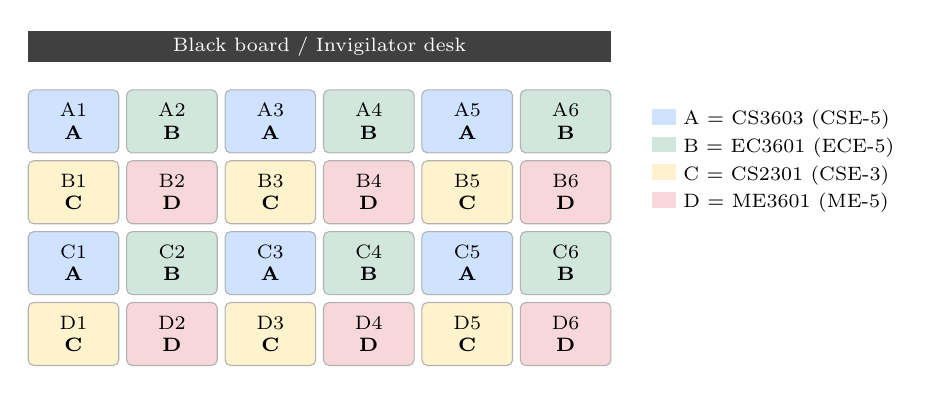
\begin{tikzpicture}[font=\scriptsize]
\definecolor{sA}{RGB}{207,226,255}
\definecolor{sB}{RGB}{209,231,221}
\definecolor{sC}{RGB}{255,243,205}
\definecolor{sD}{RGB}{248,215,218}
\fill[black!75] (0,0.35) rectangle (6*1.25-0.1,0.75);
\node[white] at (3.7,0.55) {Black board / Invigilator desk};
\foreach \s [count=\i from 0] in {A,B,A,B,A,B,C,D,C,D,C,D,A,B,A,B,A,B,C,D,C,D,C,D}{
  \pgfmathtruncatemacro{\r}{int(\i/6)}
  \pgfmathtruncatemacro{\c}{mod(\i,6)}
  \pgfmathtruncatemacro{\cc}{\c+1}
  \fill[s\s,draw=black!30,rounded corners=2pt] (\c*1.25,-\r*0.9) rectangle ++(1.15,-0.8);
  \node[align=center] at (\c*1.25+0.575,-\r*0.9-0.4) {\ifcase\r A\or B\or C\or D\fi\cc\\\textbf{\s}};
}
\node[anchor=west,align=left] at (7.8,-0.9) {
  \tikz\fill[sA](0,0)rectangle(0.3,0.2); A = CS3603 (CSE-5)\\[2pt]
  \tikz\fill[sB](0,0)rectangle(0.3,0.2); B = EC3601 (ECE-5)\\[2pt]
  \tikz\fill[sC](0,0)rectangle(0.3,0.2); C = CS2301 (CSE-3)\\[2pt]
  \tikz\fill[sD](0,0)rectangle(0.3,0.2); D = ME3601 (ME-5)};
\end{tikzpicture}

\caption{Illustrative seat pattern: no equal letters touch horizontally or vertically}\label{fig:seatex}
\end{figure}

For the single-subject slot (08-Dec-2026 14:00, CS2302, 40 students) the engine leaves alternate seats empty: 32 students in SH-01 in a chessboard pattern and 8 in LH-201, again with zero clashes.

\subsection{Complexity}
Let $P = \sum_j C_j$ be the total number of seats visited and $k$ the number of exams in the slot. Each seat calls \textsc{PickExam} at most twice, each call scans $k$ queues, so the running time is $O(P \cdot k)$ plus $O(N)$ for loading students. With $k \le 10$ and a few thousand seats the engine finishes in milliseconds; the database insert of the seats dominates. Memory use is $O(P)$ for the grid.

\subsection{Implementation}
The engine is the method \texttt{allocateSeats} of \texttt{SeatingAllocationService}. It runs in one \texttt{@Transactional} method: if any exception is thrown, the deletes of the old plan are rolled back as well.
\lstinputlisting[style=java,firstline=55,lastline=128,firstnumber=55,caption={SeatingAllocationService.allocateSeats}]{\src/service/SeatingAllocationService.java}
\lstinputlisting[style=java,firstline=130,lastline=160,firstnumber=130,caption={Neighbour-aware exam selection}]{\src/service/SeatingAllocationService.java}

\section{Invigilation Allocation Engine}
\subsection{Clash Definition}
Two duties of the same faculty member clash when they are on the same date and their half-open time intervals intersect:
\[
\mathit{clash}\big([a_s, a_e), [b_s, b_e)\big) \iff a_s < b_e \;\wedge\; b_s < a_e .
\]
This is implemented once, in the entity method \texttt{InvigilationDuty.overlaps}:
\lstinputlisting[style=java,firstline=52,lastline=54,firstnumber=52]{\src/entity/InvigilationDuty.java}
Because the intervals are half-open, a duty ending at 12:30 and another starting at 12:30 do not clash.

\subsection{Algorithm}
\begin{algorithm}[H]
\caption{Least-loaded-first invigilator assignment}
\begin{algorithmic}[1]
\Require slot date $d$, start time $t_s$
\State $seats \gets$ seat allocations of the slot; \textbf{if} empty \textbf{throw} AllocationException
\State $t_e \gets \max$ end time of the exams in the slot
\State $count[h] \gets$ number of students in each used hall $h$
\State delete existing duties of the slot; $D_f \gets$ all saved duties of each faculty $f$
\For{each used hall $h$ (ordered by name)}
  \For{$i = 1$ \textbf{to} $\max(1, \lceil count[h] / 30 \rceil)$}
    \State $cand \gets \{ f \in F : |D_f| < L_f \wedge \neg\exists x \in D_f : x.\mathrm{overlaps}(d, t_s, t_e) \}$
    \If{$cand = \emptyset$} \State \textbf{throw} AllocationException \Comment{whole transaction rolls back} \EndIf
    \State $f^* \gets \arg\min_{f \in cand} |D_f|$, ties broken by name
    \State create duty $(f^*, h, d, t_s, t_e)$; add it to $D_{f^*}$
  \EndFor
\EndFor
\State save all new duties; \Return InvigilationResult
\end{algorithmic}
\end{algorithm}

\begin{figure}[H]\centering
\resizebox{!}{0.55\textheight}{\begin{tikzpicture}[
  font=\footnotesize, node distance=0.45cm,
  term/.style={rounded rectangle,draw=egnavy,fill=egnavy,text=white,minimum height=0.7cm,minimum width=3cm},
  proc/.style={rectangle,draw=egnavy,fill=eglight,rounded corners=2pt,minimum height=0.7cm,text width=5.6cm,align=center},
  dec/.style={diamond,draw=eggold,fill=eggold!20,aspect=2.6,inner sep=1pt,text width=2.6cm,align=center},
  err/.style={rectangle,draw=red!60!black,fill=red!8,rounded corners=2pt,text width=3.0cm,align=center,minimum height=0.7cm},
  arr/.style={-{Stealth[length=2mm]},thick}]
\node[term] (s) {Start (date, startTime)};
\node[dec,below=of s] (d0) {seating exists for slot?};
\node[err,right=0.8cm of d0] (e0) {throw Allocation\-Exception};
\node[proc,below=of d0] (p1) {Count students per hall; endTime = latest end time of exams in slot};
\node[proc,below=of p1] (p2) {Delete old duties of the slot; load all faculty and all existing duties};
\node[proc,below=of p2] (p3) {For each used hall: needed = $\lceil$students / 30$\rceil$ (minimum 1)};
\node[proc,below=of p3] (p4) {Candidates = faculty with duties $<$ maxDuties \textbf{and} no duty overlapping [startTime, endTime) on that date};
\node[dec,below=of p4] (d1) {any candidate?};
\node[err,right=0.8cm of d1] (e1) {throw Allocation\-Exception (rollback)};
\node[proc,below=of d1] (p5) {Choose candidate with fewest duties (tie: name order); create duty; update workload map};
\node[dec,below=of p5] (d2) {more seats to cover?};
\node[proc,below=of d2] (p6) {saveAll duties; return InvigilationResult};
\node[term,below=of p6] (e) {End};
\draw[arr] (s)--(d0);
\draw[arr] (d0)--node[above]{no}(e0);
\draw[arr] (d0)--node[right]{yes}(p1);
\draw[arr] (p1)--(p2); \draw[arr] (p2)--(p3); \draw[arr] (p3)--(p4); \draw[arr] (p4)--(d1);
\draw[arr] (d1)--node[above]{no}(e1);
\draw[arr] (d1)--node[right]{yes}(p5);
\draw[arr] (p5)--(d2);
\draw[arr] (d2)--node[right]{no}(p6);
\draw[arr] (d2.west) -- node[above]{yes} ++(-1.3,0) |- (p4.west);
\draw[arr] (p6)--(e);
\end{tikzpicture}
}
\caption{Flowchart of the invigilation allocation engine}
\end{figure}

\subsection{Correctness Arguments}
\begin{itemize}
  \item \textbf{No clash (H4):} a faculty member is a candidate only if none of his or her duties, including the duties just created in the same run, overlaps the slot. The same person cannot be chosen twice for one slot because the first duty already overlaps.
  \item \textbf{Duty limit (H5):} candidates must have $|D_f| < L_f$.
  \item \textbf{Balance (S3):} always choosing the minimum $|D_f|$ means that a faculty member with $x+1$ duties is only chosen when nobody with $x$ duties is free. When all faculty are free, the spread $\max - \min$ is therefore at most 1.
  \item \textbf{Atomicity:} if some hall cannot be covered, an exception is thrown before \texttt{saveAll}; Spring rolls back the delete, so the previous roster stays intact.
\end{itemize}

\subsection{Worked Example on Sample Data}
Running seating and invigilation for the three sample slots in order produces 14 duties for 10 faculty:
\begin{center}
\begin{tabularx}{\linewidth}{|L{2.6cm}|L{3.6cm}|X|}
\hline\headrow\thead{Slot} & \thead{Hall (invigilators)} & \thead{Assigned faculty}\\\hline
07-Dec 09:30--12:30 & LH-101 (1), LH-201 (2), SH-01 (3) & FAC104; FAC108, FAC101; FAC106, FAC105, FAC109\\\hline
08-Dec 09:30--12:30 & LH-201 (2), SH-01 (3) & FAC103, FAC110; FAC107, FAC102, FAC104\\\hline
08-Dec 14:00--17:00 & LH-201 (1), SH-01 (2) & FAC108; FAC101, FAC106\\\hline
\end{tabularx}
\end{center}
Final workload: four faculty with 2 duties and six with 1 duty, so $\max - \min = 1$, and no faculty member appears twice in one slot. (Tie-breaking uses alphabetical order of the full name including the title, which is why ``Dr.'' names are picked before ``Prof.'' names.)

\subsection{Implementation}
\lstinputlisting[style=java,firstline=46,lastline=122,firstnumber=46,caption={InvigilationAllocationService}]{\src/service/InvigilationAllocationService.java}

\subsection{Complexity}
For $u$ used halls needing $I$ invigilators in total and $|F|$ faculty with $D$ existing duties, each pick scans all faculty and their duties: $O(I \cdot (|F| + D))$. For realistic sizes this is a few thousand operations.

\section{Exam Scheduling Rules}
\texttt{ExamService.findTimingProblem} runs before an exam is saved (both from the web form and from the REST API):
\begin{enumerate}
  \item end time must be after start time;
  \item no other exam of the same branch and semester may overlap on the same date (otherwise a student would need two seats at once).
\end{enumerate}
In the web form the problem is shown as a field error under \emph{End time}; through the API an \texttt{InvalidRequestException} is turned into HTTP 400.

\section{Validation}
Bean Validation annotations on the entities are checked with \texttt{@Valid} in both web and REST controllers.
\begin{longtable}{|p{2.3cm}|p{3.5cm}|p{7.0cm}|}
\hline\headrow\thead{Entity} & \thead{Field} & \thead{Rule (message)}\\\hline\endhead
Student & usn & \texttt{@NotBlank}, \texttt{@Pattern([A-Za-z0-9]\{6,15\})} -- USN must be 6 to 15 letters or digits; unique (checked in controller/service)\\\hline
Student & name, branch & \texttt{@NotBlank}\\\hline
Student & semester & \texttt{@Min(1)}, \texttt{@Max(8)}\\\hline
Student, Faculty & email & \texttt{@Email}\\\hline
Faculty & facultyCode, name, department & \texttt{@NotBlank}; code unique\\\hline
Faculty & maxDuties & \texttt{@Min(1)}, \texttt{@Max(20)}\\\hline
Hall & hallName, block & \texttt{@NotBlank}; name unique\\\hline
Hall & numberOfRows & \texttt{@Min(1)}, \texttt{@Max(30)}\\\hline
Hall & numberOfColumns & \texttt{@Min(1)}, \texttt{@Max(20)}\\\hline
Exam & subjectCode, subjectName, branch & \texttt{@NotBlank}\\\hline
Exam & examDate, startTime, endTime & \texttt{@NotNull}; plus timing rules of Section 5\\\hline
\end{longtable}

\section{Exception Handling}
\subsection{Custom Exceptions}
\begin{tabularx}{\linewidth}{|L{4.6cm}|X|l|}
\hline\headrow\thead{Exception} & \thead{Thrown when} & \thead{HTTP}\\\hline
ResourceNotFoundException & id, USN or faculty code does not exist & 404\\\hline
DuplicateResourceException & USN, faculty code or hall name already exists & 409\\\hline
InsufficientCapacityException & students in slot $>$ total hall seats; carries \texttt{required} and \texttt{available} & 422\\\hline
AllocationException & no exams in slot, no students, seating missing before invigilation, not enough free faculty, no plan for PDF & 422\\\hline
InvalidRequestException & exam timing rule broken & 400\\\hline
MethodArgumentNotValidException (Spring) & Bean Validation fails on a JSON body & 400\\\hline
MethodArgumentTypeMismatch, MissingServletRequestParameter, HttpMessageNotReadable (Spring) & bad date/time format, missing parameter, malformed JSON & 400\\\hline
AccessDeniedException (Spring) & faculty asks for another faculty's roster & 403\\\hline
Any other Exception & unexpected failure; details are not leaked & 500\\\hline
\end{tabularx}

\subsection{Two Centralized Handlers}
\begin{itemize}
  \item \texttt{ApiExceptionHandler} -- \texttt{@RestControllerAdvice} restricted with \texttt{basePackages} to \texttt{controller.api}, returns an \texttt{ErrorResponse} record as JSON.
  \item \texttt{WebExceptionHandler} -- \texttt{@ControllerAdvice} restricted to \texttt{controller.web}, renders \texttt{error/app-error.html} with status, title and message.
\end{itemize}
Restricting each advice by package ensures that a browser user never sees raw JSON and an API client never receives an HTML page.

\lstinputlisting[style=java,firstline=22,lastline=76,firstnumber=22,caption={ApiExceptionHandler}]{\src/exception/ApiExceptionHandler.java}

\noindent Example error body:
\begin{lstlisting}[style=json]
{
  "timestamp": "2026-12-01T10:15:30",
  "status": 422,
  "error": "Unprocessable Entity",
  "message": "Insufficient hall capacity: 148 students need seats but only 36 seats are available",
  "path": "/api/allocations/seating",
  "fieldErrors": null
}
\end{lstlisting}

\section{Transaction Management}
\begin{tabularx}{\linewidth}{|L{5cm}|X|}
\hline\headrow\thead{Method} & \thead{Transaction behaviour}\\\hline
allocateSeats, allocateInvigilators & Read-write; bulk delete of old slot data and batch insert of new data commit together or roll back together.\\\hline
create / update / delete in CRUD services & Read-write; e.g. deleting a student deletes seat rows and login account in the same transaction.\\\hline
find* methods & \texttt{readOnly = true}; Hibernate skips dirty checking.\\\hline
\end{tabularx}
Bulk deletes are written as JPQL \texttt{@Modifying} queries (\texttt{delete from SeatAllocation s where \ldots}) so that one SQL statement removes a whole slot instead of loading every row first.

\section{Security Specification}
\subsection{Filter Chains}
\lstinputlisting[style=java,firstline=29,lastline=68,firstnumber=29,caption={SecurityConfig}]{\src/security/SecurityConfig.java}

\subsection{Access Control Matrix}
\begin{tabularx}{\linewidth}{|X|c|c|c|c|}
\hline\headrow\thead{Resource} & \thead{Guest} & \thead{STUDENT} & \thead{FACULTY} & \thead{ADMIN}\\\hline
/, /login, /seat-lookup, static files & \checkmark & \checkmark & \checkmark & \checkmark\\\hline
/student/seat & -- & \checkmark & -- & --\\\hline
/faculty/duties & -- & -- & \checkmark & --\\\hline
/admin/** (pages and PDF reports) & -- & -- & -- & \checkmark\\\hline
GET /api/seats/\{usn\} & \checkmark & \checkmark & \checkmark & \checkmark\\\hline
GET /api/duties/faculty/\{code\} & -- & -- & own code only & \checkmark\\\hline
all other /api/** & -- & -- & -- & \checkmark\\\hline
\end{tabularx}

\subsection{Authentication Flow}
\begin{enumerate}
  \item The login form posts \texttt{username}, \texttt{password} and the CSRF token to \texttt{/login}.
  \item \texttt{AppUserDetailsService.loadUserByUsername} reads \texttt{app\_users} (case-insensitive) and builds a Spring \texttt{User} with authority \texttt{ROLE\_<role>}.
  \item \texttt{BCryptPasswordEncoder.matches} compares the password with the stored hash.
  \item On success the session id is changed (fixation protection) and the user is redirected to \texttt{/dashboard}, which forwards by role.
  \item On failure the user returns to \texttt{/login?error}; the message does not reveal whether the username exists.
\end{enumerate}

\subsection{Account Provisioning}
When the exam cell adds a student or faculty member, \texttt{UserAccountService} creates an \texttt{AppUser} with the USN or faculty code as username, the default password \texttt{Welcome@123} (BCrypt-hashed) and the matching role. Deleting the person deletes the account in the same transaction. The admin account (\texttt{admin}/\texttt{admin123}) is created by \texttt{DataSeeder} on first start and should be changed before real use.

\section{PDF Report Generation}
\texttt{ReportPdfService} uses OpenPDF to build documents in memory (\texttt{ByteArrayOutputStream}) and the controller streams the bytes with \texttt{Content-Type: application/pdf}.
\begin{itemize}
  \item \textbf{Seating chart} (A4 landscape): for each hall one page with a table of \emph{columns} cells per row, each cell showing seat label, USN and subject code in the subject colour; followed by one attendance sheet page (Sl, Seat, Name, USN, Subject, Signature).
  \item \textbf{Duty roster} (A4 portrait): Sl, Date, Time, Faculty (code), Department, Hall, Signature; for one date or for all dates.
\end{itemize}

\section{Configuration Parameters}
\begin{tabularx}{\linewidth}{|L{5.6cm}|L{3.6cm}|X|}
\hline\headrow\thead{Property} & \thead{Default} & \thead{Meaning}\\\hline
spring.datasource.url & \url{jdbc:mysql://localhost:3306/examgrid_db} & MySQL connection, database created if missing\\\hline
spring.jpa.hibernate.ddl-auto & update & Create or update tables from entities\\\hline
spring.jpa.open-in-view & false & No lazy loading in views\\\hline
server.servlet.session.timeout & 30m & Idle session timeout\\\hline
examgrid.students-per-invigilator & 30 & Students per invigilator in a hall\\\hline
examgrid.seed-sample-data & true & Load demo data when the student table is empty\\\hline
\end{tabularx}

\end{document}
